\section{Participant 1}

%% AS

\subsection{Date \& Time}
\begin{table}[ht]
  \begin{tabular}{|P{3cm}|P{3cm}|}
	\multicolumn{2}{c}{\textbf{2016-07-28}}    	\\ \hline
    Start Time      			& End Time   					\\ \hline
   \textbf{12:52:44} 	& \textbf{13:04:45}    	\\ \hline
   \multicolumn{2}{c}{Duration}    						\\ \hline
   \multicolumn{2}{c}{\textbf{00:12:01}} 			\\ \hline
  \end{tabular}
  \newline\newline
 \caption{P1: Date and Time}\label{dandt1}
\end{table}

\subsection{Questions}
\begin{itemize} 
  \item[\Checkmark] Are you a Student?
  \item[\XSolidBrush] Did you work in a team?
  \item[\Checkmark] Did you listen to music?
  \item[\XSolidBrush] Did you feel tired?
  \item[\Checkmark] Did you enjoy the tasks?
  \item[\Checkmark] Did you give all you attention to the tasks?
  \item[\XSolidBrush] Were you distracted during the tasks?
  \item[\XSolidBrush] Did you feel stressed
  \item[\XSolidBrush] Do you think the tasks were easy?  
\end{itemize}


\FloatBarrier
\newpage
\subsection{Accelerometer}

\begin{figure}[ht]
	\centering
	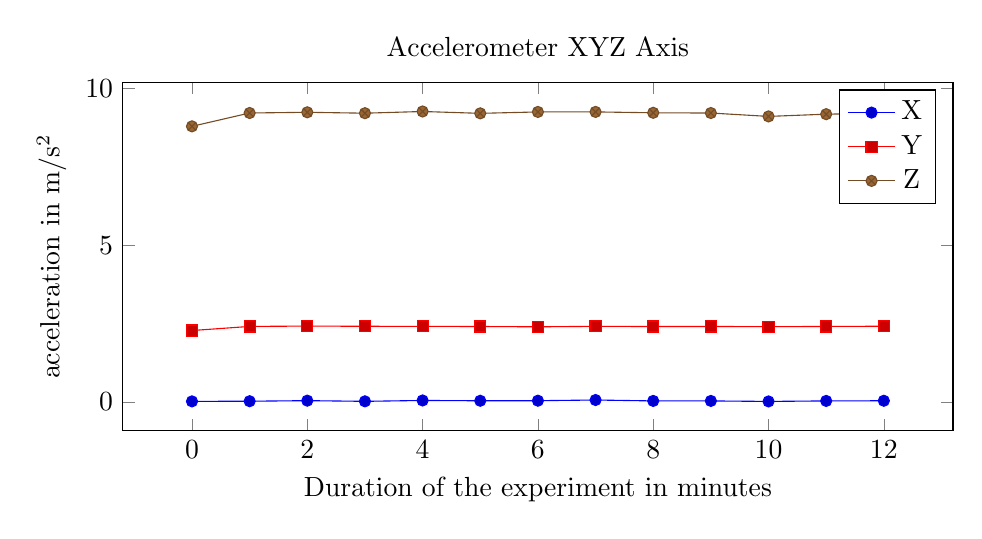
\begin{tikzpicture}
\begin{axis}[
	height=6cm,
	width=\textwidth,
	xlabel=Duration of the experiment in minutes,
	ylabel=acceleration in m/s$^2$,
	title=Accelerometer XYZ Axis,
	unbounded coords=discard],
	
%X
\addplot coordinates {
(0 , 0.019438637881)
(1 , 0.0247400849444)
(2 , 0.0424115735714)
(3 , 0.02101577)
(4 , 0.0486535994286)
(5 , 0.0389057787143)
(6 , 0.041366485)
(7 , 0.0629475533333)
(8 , 0.034117374125)
(9 , 0.033618582)
(10 , 0.0179565136667)
(11 , 0.0341173747143)
(12 , 0.038905777)
};

%Y
\addplot coordinates {
(0 , 2.2777979)
(1 , 2.40836742222)
(2 , 2.42019587143)
(3 , 2.41288974444)
(4 , 2.41164518571)
(5 , 2.40600168571)
(6 , 2.39666241111)
(7 , 2.4114599)
(8 , 2.4058734375)
(9 , 2.40826766667)
(10 , 2.3990899)
(11 , 2.40848141429)
(12 , 2.4145525)
};

%Z
\addplot coordinates {
(0 , 8.7865777619)
(1 , 9.21202333333)
(2 , 9.234265)
(3 , 9.20590511111)
(4 , 9.26008828571)
(5 , 9.20108792857)
(6 , 9.24580855556)
(7 , 9.24680616667)
(8 , 9.2185745)
(9 , 9.21099291667)
(10 , 9.1032535)
(11 , 9.17449528571)
(12 , 9.20391)
};

\addlegendentry{X}
\addlegendentry{Y}
\addlegendentry{Z}
\end{axis}
\end{tikzpicture}
 	\vspace{5 mm}
\end{figure}

\FloatBarrier
\subsection{Light Level}
\begin{figure}[ht]
	\centering
	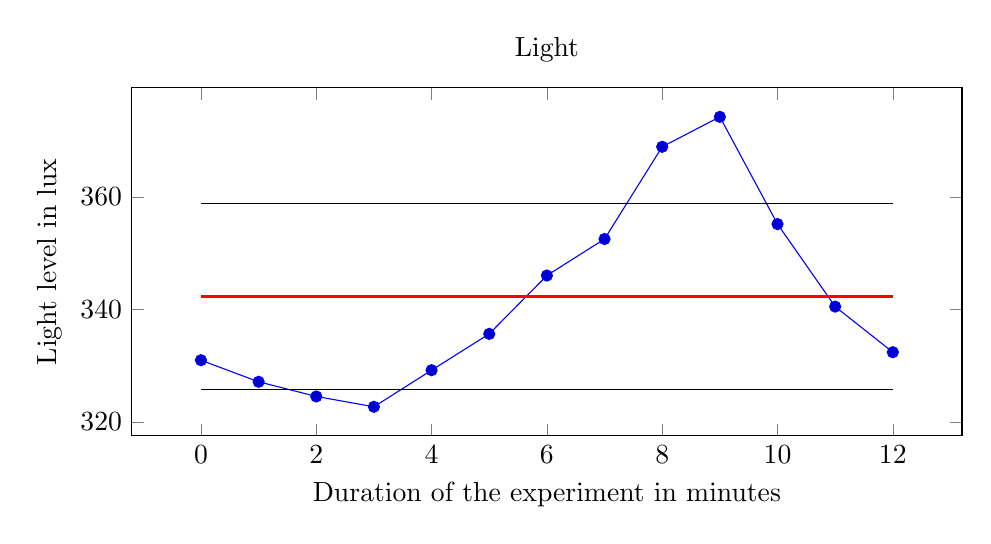
\begin{tikzpicture}
\begin{axis}[
	height=6cm,
	width=\textwidth,
	xlabel=Duration of the experiment in minutes,
	ylabel=Light level in lux,
	title=Light,
	unbounded coords=discard],
	
\addplot coordinates {
(0 , 330.986057143)
(1 , 327.141866667)
(2 , 324.539771429)
(3 , 322.701066667)
(4 , 329.208342857)
(5 , 335.669942857)
(6 , 346.047466667)
(7 , 352.541066667)
(8 , 368.9453)
(9 , 374.263066667)
(10 , 355.196133333)
(11 , 340.515885714)
(12 , 332.4064)
};

\addplot[mark=none, red, very thick] coordinates {(0,342.312997222) (12,342.312997222)};

\addplot[mark=none, black] coordinates {(0,325.748247381) (12,325.748247381)};
\addplot[mark=none, black] coordinates {(0,358.877747063) (12,358.877747063)};

\end{axis}
\end{tikzpicture}
 	\vspace{5 mm}
\end{figure}

\newpage
\FloatBarrier
\newpage
\subsection{Noise Level}
\begin{figure}[ht]
	\centering
	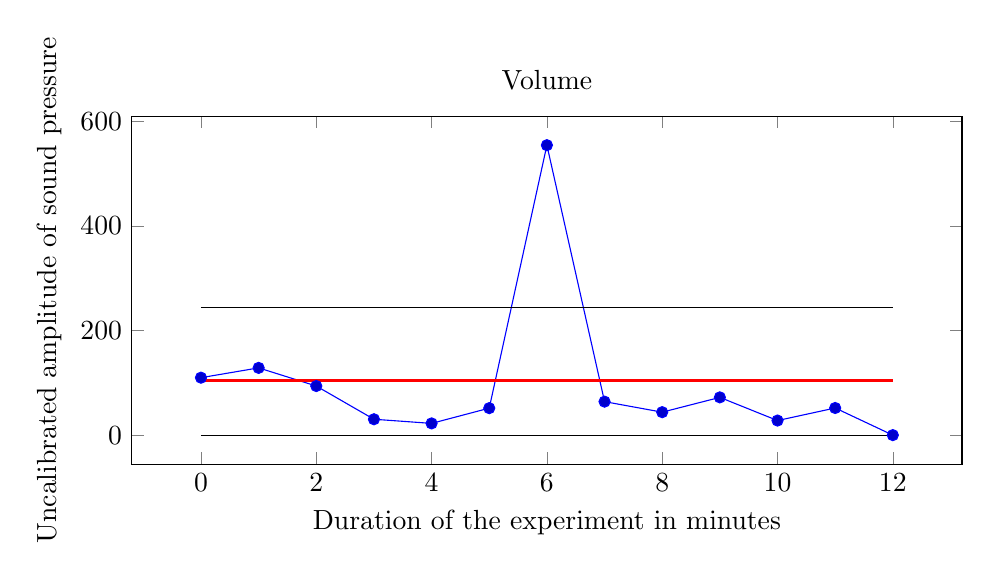
\begin{tikzpicture}
\begin{axis}[
	height=6cm,
	width=\textwidth,
	ylabel=Uncalibrated amplitude of sound pressure,
	xlabel=Duration of the experiment in minutes,
	title=Volume,
	unbounded coords=discard],

\addplot coordinates {
(0 , 109.80952381)
(1 , 128.555555556)
(2 , 93.8571428571)
(3 , 30.3333333333)
(4 , 22.4285714286)
(5 , 51.5714285714)
(6 , 554.333333333)
(7 , 64.0)
(8 , 43.875)
(9 , 72.1666666667)
(10 , 27.8333333333)
(11 , 51.8571428571)
(12 , 0.0)
};

\addplot[mark=none, red, very thick] coordinates {(0,104.218419312) (12,104.218419312)};

\addplot[mark=none, black] coordinates {(0, 0) (12, 0)};
\addplot[mark=none, black] coordinates {(0, 243.597156419) (12, 243.597156419)};

\end{axis}
\end{tikzpicture}
 	\vspace{5 mm}
\end{figure}

\FloatBarrier

\subsection{Location}
No data gathered

\FloatBarrier